% Created by tikzDevice version 0.12 on 2019-04-30 20:46:52
% !TEX encoding = UTF-8 Unicode
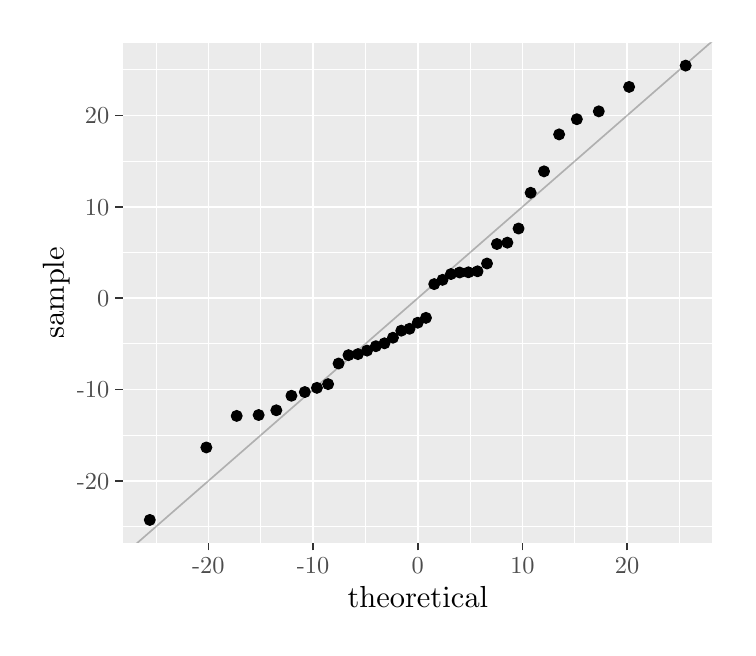
\begin{tikzpicture}[x=1pt,y=1pt]
\definecolor{fillColor}{RGB}{255,255,255}
\path[use as bounding box,fill=fillColor,fill opacity=0.00] (0,0) rectangle (252.94,216.81);
\begin{scope}
\path[clip] (  0.00,  0.00) rectangle (252.94,216.81);
\definecolor{drawColor}{RGB}{255,255,255}
\definecolor{fillColor}{RGB}{255,255,255}

\path[draw=drawColor,line width= 0.6pt,line join=round,line cap=round,fill=fillColor] (  0.00,  0.00) rectangle (252.94,216.81);
\end{scope}
\begin{scope}
\path[clip] ( 34.45, 30.72) rectangle (247.44,211.31);
\definecolor{fillColor}{gray}{0.92}

\path[fill=fillColor] ( 34.45, 30.72) rectangle (247.44,211.31);
\definecolor{drawColor}{RGB}{255,255,255}

\path[draw=drawColor,line width= 0.3pt,line join=round] ( 34.45, 36.51) --
	(247.44, 36.51);

\path[draw=drawColor,line width= 0.3pt,line join=round] ( 34.45, 69.53) --
	(247.44, 69.53);

\path[draw=drawColor,line width= 0.3pt,line join=round] ( 34.45,102.55) --
	(247.44,102.55);

\path[draw=drawColor,line width= 0.3pt,line join=round] ( 34.45,135.56) --
	(247.44,135.56);

\path[draw=drawColor,line width= 0.3pt,line join=round] ( 34.45,168.58) --
	(247.44,168.58);

\path[draw=drawColor,line width= 0.3pt,line join=round] ( 34.45,201.59) --
	(247.44,201.59);

\path[draw=drawColor,line width= 0.3pt,line join=round] ( 46.36, 30.72) --
	( 46.36,211.31);

\path[draw=drawColor,line width= 0.3pt,line join=round] ( 84.20, 30.72) --
	( 84.20,211.31);

\path[draw=drawColor,line width= 0.3pt,line join=round] (122.03, 30.72) --
	(122.03,211.31);

\path[draw=drawColor,line width= 0.3pt,line join=round] (159.87, 30.72) --
	(159.87,211.31);

\path[draw=drawColor,line width= 0.3pt,line join=round] (197.70, 30.72) --
	(197.70,211.31);

\path[draw=drawColor,line width= 0.3pt,line join=round] (235.54, 30.72) --
	(235.54,211.31);

\path[draw=drawColor,line width= 0.6pt,line join=round] ( 34.45, 53.02) --
	(247.44, 53.02);

\path[draw=drawColor,line width= 0.6pt,line join=round] ( 34.45, 86.04) --
	(247.44, 86.04);

\path[draw=drawColor,line width= 0.6pt,line join=round] ( 34.45,119.05) --
	(247.44,119.05);

\path[draw=drawColor,line width= 0.6pt,line join=round] ( 34.45,152.07) --
	(247.44,152.07);

\path[draw=drawColor,line width= 0.6pt,line join=round] ( 34.45,185.08) --
	(247.44,185.08);

\path[draw=drawColor,line width= 0.6pt,line join=round] ( 65.28, 30.72) --
	( 65.28,211.31);

\path[draw=drawColor,line width= 0.6pt,line join=round] (103.11, 30.72) --
	(103.11,211.31);

\path[draw=drawColor,line width= 0.6pt,line join=round] (140.95, 30.72) --
	(140.95,211.31);

\path[draw=drawColor,line width= 0.6pt,line join=round] (178.78, 30.72) --
	(178.78,211.31);

\path[draw=drawColor,line width= 0.6pt,line join=round] (216.62, 30.72) --
	(216.62,211.31);
\definecolor{drawColor}{RGB}{0,0,0}
\definecolor{fillColor}{RGB}{0,0,0}

\path[draw=drawColor,line width= 0.4pt,line join=round,line cap=round,fill=fillColor] ( 44.13, 38.93) circle (  1.96);

\path[draw=drawColor,line width= 0.4pt,line join=round,line cap=round,fill=fillColor] ( 64.57, 65.12) circle (  1.96);

\path[draw=drawColor,line width= 0.4pt,line join=round,line cap=round,fill=fillColor] ( 75.53, 76.52) circle (  1.96);

\path[draw=drawColor,line width= 0.4pt,line join=round,line cap=round,fill=fillColor] ( 83.46, 76.84) circle (  1.96);

\path[draw=drawColor,line width= 0.4pt,line join=round,line cap=round,fill=fillColor] ( 89.85, 78.55) circle (  1.96);

\path[draw=drawColor,line width= 0.4pt,line join=round,line cap=round,fill=fillColor] ( 95.31, 83.80) circle (  1.96);

\path[draw=drawColor,line width= 0.4pt,line join=round,line cap=round,fill=fillColor] (100.14, 85.14) circle (  1.96);

\path[draw=drawColor,line width= 0.4pt,line join=round,line cap=round,fill=fillColor] (104.52, 86.66) circle (  1.96);

\path[draw=drawColor,line width= 0.4pt,line join=round,line cap=round,fill=fillColor] (108.56, 88.00) circle (  1.96);

\path[draw=drawColor,line width= 0.4pt,line join=round,line cap=round,fill=fillColor] (112.34, 95.45) circle (  1.96);

\path[draw=drawColor,line width= 0.4pt,line join=round,line cap=round,fill=fillColor] (115.92, 98.47) circle (  1.96);

\path[draw=drawColor,line width= 0.4pt,line join=round,line cap=round,fill=fillColor] (119.34, 98.85) circle (  1.96);

\path[draw=drawColor,line width= 0.4pt,line join=round,line cap=round,fill=fillColor] (122.63,100.12) circle (  1.96);

\path[draw=drawColor,line width= 0.4pt,line join=round,line cap=round,fill=fillColor] (125.82,101.71) circle (  1.96);

\path[draw=drawColor,line width= 0.4pt,line join=round,line cap=round,fill=fillColor] (128.93,102.75) circle (  1.96);

\path[draw=drawColor,line width= 0.4pt,line join=round,line cap=round,fill=fillColor] (131.99,104.77) circle (  1.96);

\path[draw=drawColor,line width= 0.4pt,line join=round,line cap=round,fill=fillColor] (135.00,107.32) circle (  1.96);

\path[draw=drawColor,line width= 0.4pt,line join=round,line cap=round,fill=fillColor] (137.98,108.00) circle (  1.96);

\path[draw=drawColor,line width= 0.4pt,line join=round,line cap=round,fill=fillColor] (140.95,110.20) circle (  1.96);

\path[draw=drawColor,line width= 0.4pt,line join=round,line cap=round,fill=fillColor] (143.92,111.95) circle (  1.96);

\path[draw=drawColor,line width= 0.4pt,line join=round,line cap=round,fill=fillColor] (146.90,124.15) circle (  1.96);

\path[draw=drawColor,line width= 0.4pt,line join=round,line cap=round,fill=fillColor] (149.91,125.69) circle (  1.96);

\path[draw=drawColor,line width= 0.4pt,line join=round,line cap=round,fill=fillColor] (152.96,127.78) circle (  1.96);

\path[draw=drawColor,line width= 0.4pt,line join=round,line cap=round,fill=fillColor] (156.08,128.34) circle (  1.96);

\path[draw=drawColor,line width= 0.4pt,line join=round,line cap=round,fill=fillColor] (159.27,128.41) circle (  1.96);

\path[draw=drawColor,line width= 0.4pt,line join=round,line cap=round,fill=fillColor] (162.56,128.77) circle (  1.96);

\path[draw=drawColor,line width= 0.4pt,line join=round,line cap=round,fill=fillColor] (165.98,131.59) circle (  1.96);

\path[draw=drawColor,line width= 0.4pt,line join=round,line cap=round,fill=fillColor] (169.56,138.63) circle (  1.96);

\path[draw=drawColor,line width= 0.4pt,line join=round,line cap=round,fill=fillColor] (173.34,139.13) circle (  1.96);

\path[draw=drawColor,line width= 0.4pt,line join=round,line cap=round,fill=fillColor] (177.38,144.23) circle (  1.96);

\path[draw=drawColor,line width= 0.4pt,line join=round,line cap=round,fill=fillColor] (181.75,157.15) circle (  1.96);

\path[draw=drawColor,line width= 0.4pt,line join=round,line cap=round,fill=fillColor] (186.58,164.89) circle (  1.96);

\path[draw=drawColor,line width= 0.4pt,line join=round,line cap=round,fill=fillColor] (192.04,178.24) circle (  1.96);

\path[draw=drawColor,line width= 0.4pt,line join=round,line cap=round,fill=fillColor] (198.44,183.73) circle (  1.96);

\path[draw=drawColor,line width= 0.4pt,line join=round,line cap=round,fill=fillColor] (206.37,186.57) circle (  1.96);

\path[draw=drawColor,line width= 0.4pt,line join=round,line cap=round,fill=fillColor] (217.33,195.40) circle (  1.96);

\path[draw=drawColor,line width= 0.4pt,line join=round,line cap=round,fill=fillColor] (237.76,203.10) circle (  1.96);
\definecolor{drawColor}{RGB}{0,0,0}

\path[draw=drawColor,draw opacity=0.25,line width= 0.6pt,line join=round] ( 34.45, 26.12) -- (247.44,211.98);
\end{scope}
\begin{scope}
\path[clip] (  0.00,  0.00) rectangle (252.94,216.81);
\definecolor{drawColor}{gray}{0.30}

\node[text=drawColor,anchor=base east,inner sep=0pt, outer sep=0pt, scale=  0.88] at ( 29.50, 49.99) {-20};

\node[text=drawColor,anchor=base east,inner sep=0pt, outer sep=0pt, scale=  0.88] at ( 29.50, 83.01) {-10};

\node[text=drawColor,anchor=base east,inner sep=0pt, outer sep=0pt, scale=  0.88] at ( 29.50,116.02) {0};

\node[text=drawColor,anchor=base east,inner sep=0pt, outer sep=0pt, scale=  0.88] at ( 29.50,149.04) {10};

\node[text=drawColor,anchor=base east,inner sep=0pt, outer sep=0pt, scale=  0.88] at ( 29.50,182.05) {20};
\end{scope}
\begin{scope}
\path[clip] (  0.00,  0.00) rectangle (252.94,216.81);
\definecolor{drawColor}{gray}{0.20}

\path[draw=drawColor,line width= 0.6pt,line join=round] ( 31.70, 53.02) --
	( 34.45, 53.02);

\path[draw=drawColor,line width= 0.6pt,line join=round] ( 31.70, 86.04) --
	( 34.45, 86.04);

\path[draw=drawColor,line width= 0.6pt,line join=round] ( 31.70,119.05) --
	( 34.45,119.05);

\path[draw=drawColor,line width= 0.6pt,line join=round] ( 31.70,152.07) --
	( 34.45,152.07);

\path[draw=drawColor,line width= 0.6pt,line join=round] ( 31.70,185.08) --
	( 34.45,185.08);
\end{scope}
\begin{scope}
\path[clip] (  0.00,  0.00) rectangle (252.94,216.81);
\definecolor{drawColor}{gray}{0.20}

\path[draw=drawColor,line width= 0.6pt,line join=round] ( 65.28, 27.97) --
	( 65.28, 30.72);

\path[draw=drawColor,line width= 0.6pt,line join=round] (103.11, 27.97) --
	(103.11, 30.72);

\path[draw=drawColor,line width= 0.6pt,line join=round] (140.95, 27.97) --
	(140.95, 30.72);

\path[draw=drawColor,line width= 0.6pt,line join=round] (178.78, 27.97) --
	(178.78, 30.72);

\path[draw=drawColor,line width= 0.6pt,line join=round] (216.62, 27.97) --
	(216.62, 30.72);
\end{scope}
\begin{scope}
\path[clip] (  0.00,  0.00) rectangle (252.94,216.81);
\definecolor{drawColor}{gray}{0.30}

\node[text=drawColor,anchor=base,inner sep=0pt, outer sep=0pt, scale=  0.88] at ( 65.28, 19.71) {-20};

\node[text=drawColor,anchor=base,inner sep=0pt, outer sep=0pt, scale=  0.88] at (103.11, 19.71) {-10};

\node[text=drawColor,anchor=base,inner sep=0pt, outer sep=0pt, scale=  0.88] at (140.95, 19.71) {0};

\node[text=drawColor,anchor=base,inner sep=0pt, outer sep=0pt, scale=  0.88] at (178.78, 19.71) {10};

\node[text=drawColor,anchor=base,inner sep=0pt, outer sep=0pt, scale=  0.88] at (216.62, 19.71) {20};
\end{scope}
\begin{scope}
\path[clip] (  0.00,  0.00) rectangle (252.94,216.81);
\definecolor{drawColor}{RGB}{0,0,0}

\node[text=drawColor,anchor=base,inner sep=0pt, outer sep=0pt, scale=  1.10] at (140.95,  7.44) {theoretical};
\end{scope}
\begin{scope}
\path[clip] (  0.00,  0.00) rectangle (252.94,216.81);
\definecolor{drawColor}{RGB}{0,0,0}

\node[text=drawColor,rotate= 90.00,anchor=base,inner sep=0pt, outer sep=0pt, scale=  1.10] at ( 13.08,121.02) {sample};
\end{scope}
\end{tikzpicture}
